\section{Architectural Evolution}

The popularity of microservices and containerization has exploded in recent
years. The need for scalable, easily deployable applications has led to 
abandoning monolithic architectures, where all processes are tightly coupled
and run as a single service, in favor of microservices. Microservices are an
architectural and organizational approach for software development where software
is composed of small independent services that communicate over well-defined
APIs.

The current industry trend for microservices is to use containerization to
deliver smaller, single-function modules, which work together to create more
agile, scalable applications. Containerization is a form of virtualization where
applications run in isolated user spaces, called containers, while using the
same shared operating system. A container is essentially a fully packaged and
portable computing environment. Everything an application needs to run --its
binaries, libraries, configuration files, and dependencies-- are encapsulated and
isolated in their container.

The extensive use of containers has driven the need to automate containers'
deployment and management. Container orchestration automates the operational
effort required to run containerized workloads and services. Container
orchestration includes various actions software teams need to manage a
container's lifecycle, including provisioning, deployment, scaling (up and
down), networking, load balancing, and more.

Kubernetes is the most popular solution among various container orchestrators
and has become the industry standard. Initially launched by Google, Kubernetes
is a portable, extensible, open-source platform for managing containerized
workloads and services that facilitates declarative configuration and
automation.

\begin{figure}
    \centering
    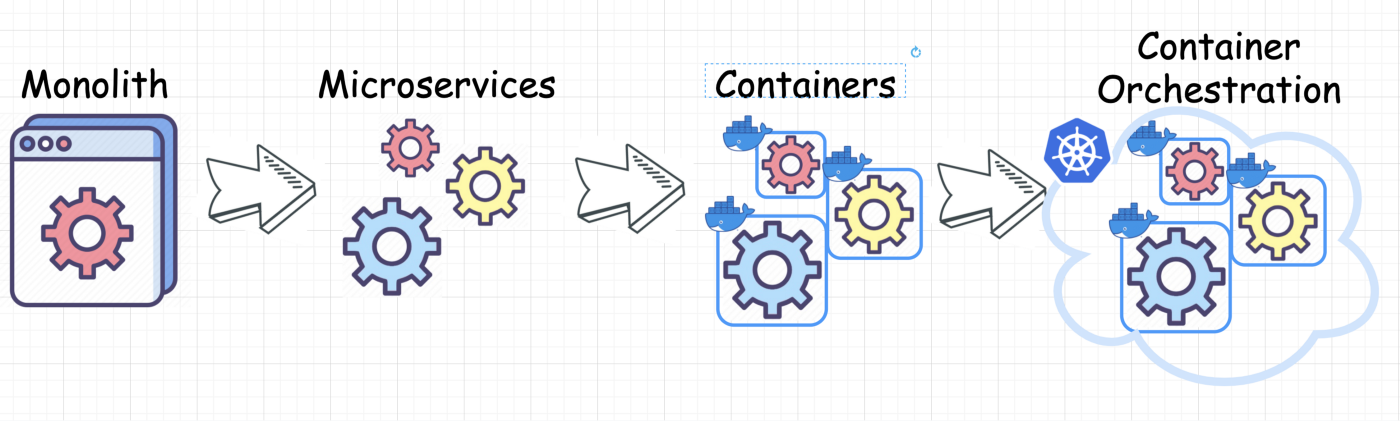
\includegraphics[width=0.8\textwidth]{resources/containerization.png}
    \caption{Architectural evolution: From monolithic applications to containerized microservices that are managed by a container orchestrator}
\end{figure}

Kubernetes operates on a cluster. A Kubernetes cluster is a set of node machines
for running containerized applications. The cluster is the heart of Kubernetes'
key advantage: the ability to schedule and run containers across a group of
machines, be they physical or virtual, on-premises or in the cloud.
